\documentclass[10pt,a4paper]{article}
\usepackage[margin=2cm]{geometry}
\usepackage{amsmath,amssymb}
\usepackage{graphicx,booktabs,xcolor}
\usepackage{listings}
\usepackage{tikz}
\usepackage[colorlinks=true,linkcolor=blue!50!black,urlcolor=blue!50!black,citecolor=blue!50!black]{hyperref}
\usepackage{microtype}

\lstset{language=Python,basicstyle=\ttfamily\small,keywordstyle=\color{blue!60!black}\bfseries,
  commentstyle=\color{green!40!black},stringstyle=\color{red!50!black},
  frame=single,framerule=0.3pt,rulecolor=\color{gray!60},backgroundcolor=\color{gray!5},
  columns=fullflexible,keepspaces=true,showstringspaces=false,
  numbers=left,numberstyle=\tiny\color{gray},xleftmargin=1.5em,aboveskip=6pt,belowskip=4pt}
\newcommand{\code}[1]{\texttt{#1}}
\newcommand{\PP}{\mathcal{P}}
\renewcommand{\labelitemi}{$\bullet$}
\setlength{\parindent}{0pt}\setlength{\parskip}{4pt}\setlength{\emergencystretch}{3em}\sloppy
\setlength{\textfloatsep}{8pt}\setlength{\intextsep}{7pt}\setlength{\abovecaptionskip}{4pt}\setlength{\belowcaptionskip}{0pt}

\newcommand{\orderpic}{%
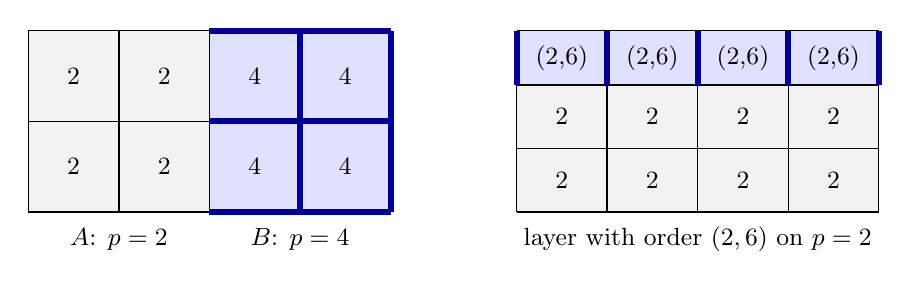
\begin{tikzpicture}[x=1.15cm,y=1.15cm,
  lo/.style={line width=0.5pt},hi/.style={line width=2.2pt,blue!60!black},
  lab/.style={font=\small}]
% left: two regions
\fill[gray!10] (0,0) rectangle (2,2);
\fill[blue!12] (2,0) rectangle (4,2);
\foreach \x in {0,1,2} \draw[lo] (\x,0)--(\x,2);
\foreach \y in {0,1,2} \draw[lo] (0,\y)--(2,\y);
\foreach \x in {3,4} \draw[hi] (\x,0)--(\x,2);
\foreach \y in {0,1,2} \draw[hi] (2,\y)--(4,\y);
\foreach \x in {0.5,1.5} \foreach \y in {0.5,1.5} \node[lab] at (\x,\y) {2};
\foreach \x in {2.5,3.5} \foreach \y in {0.5,1.5} \node[lab] at (\x,\y) {4};
\node[lab] at (1,-0.3) {$A$: $p=2$};
\node[lab] at (3,-0.3) {$B$: $p=4$};
% right: anisotropic layer
\begin{scope}[xshift=6.2cm]
\fill[gray!10] (0,0) rectangle (4,1.4);
\fill[blue!12] (0,1.4) rectangle (4,2);
\foreach \x in {0,1,2,3,4} \draw[lo] (\x,0)--(\x,1.4);
\foreach \y in {0,0.7,1.4,2} \draw[lo] (0,\y)--(4,\y);
\foreach \x in {0,1,2,3,4} \draw[hi] (\x,1.4)--(\x,2);
\foreach \x in {0.5,1.5,2.5,3.5} { \node[lab] at (\x,0.35) {2}; \node[lab] at (\x,1.05) {2}; \node[lab] at (\x,1.7) {(2,6)}; }
\node[lab] at (2,-0.3) {layer with order $(2,6)$ on $p=2$};
\end{scope}
\end{tikzpicture}}
%html \renewcommand{\orderpic}{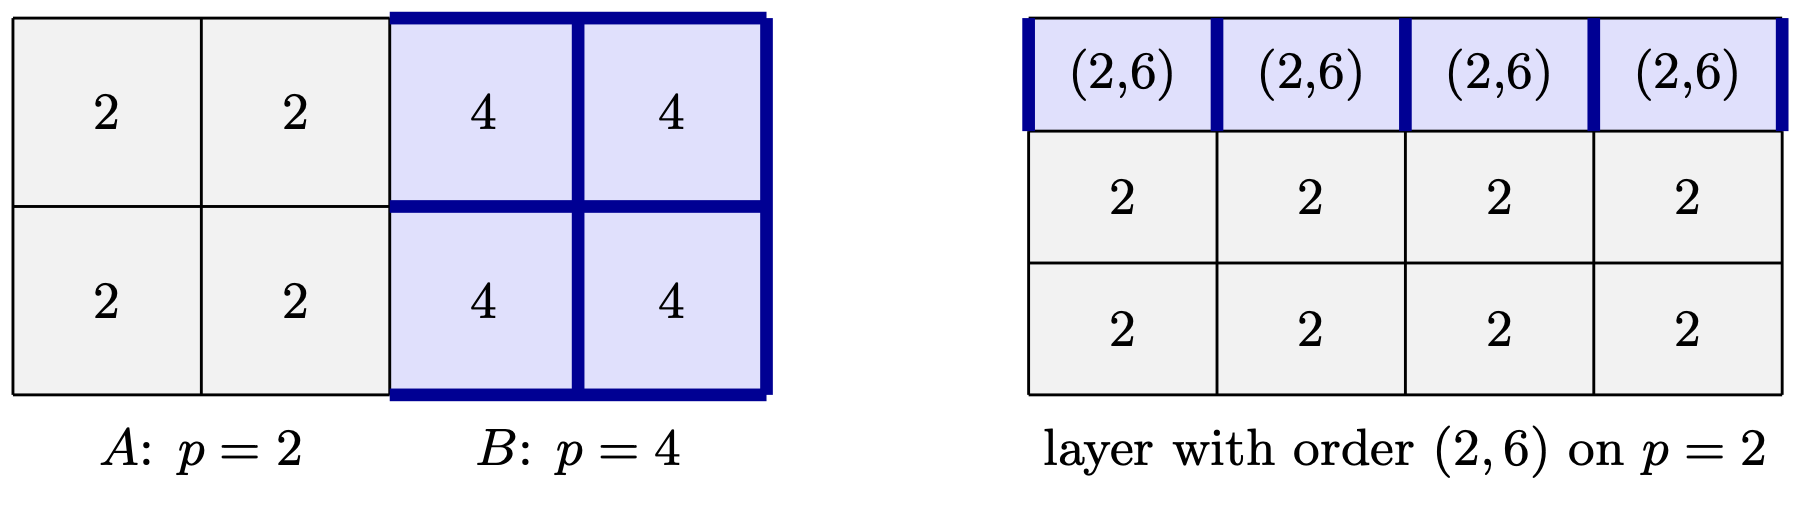
\includegraphics[width=0.9\textwidth]{orders.png}}

\title{\vspace{-1.2cm}Variable Polynomial Order\\[2pt]
\large One order specification for all spaces: regions, elements, the minimum rule, and linked spaces}
\author{Christopher Lackner \and Edoardo Bonetti \and Astrid Pechstein \and Joachim Sch\"oberl}
\date{NGSolve Technical Note 2026-09\quad$\bullet$\quad version 2026-11-23\quad$\bullet$\quad implemented for H1 and L2}

\begin{document}
\maketitle\vspace{-1.2cm}

\section{The problem}

The high order spaces of NGSolve \cite{s14} carry an individual polynomial order on every edge, face and cell \cite{sz05,z06}. The elements support this well; the way the orders are \emph{set} has grown over twenty years and no longer fits together. The order information of an $H^1$ space lives in four places: the flags of the constructor (\code{order}, \code{orderinner}, \code{orderface}, \code{orderedge}, \code{trigorder}, \dots, \code{relorder}, \code{variableorder}, \code{order\_policy}), an order increment per element shape, the arrays of edge, face and cell orders which \code{SetOrder(NodeId, p)} writes into, and the element orders stored in the Netgen mesh. The arrays are input and derived data at the same time. The consequences:
\begin{itemize}\setlength\itemsep{1pt}
\item Orders set per node are lost when the mesh is refined, and when \code{SetOrder(ET, p)} is called afterwards. In the opposite sequence the second call throws.
\item \code{order\_policy=CONSTANT} together with \code{orderinner}, or with a later \code{SetOrder(ET, p)}, returns elements which do not match the dof numbers. Without this flag the fast fixed order elements are never used.
\item Setting the order of a cell leaves its edges and faces untouched; conformity is the user's task. Only the \code{variableorder} mode derives them, by the maximum rule.
\item Anisotropic orders are given in the axes of the reference element. One has to know the local vertex numbering; on simplices and pyramids two of the three numbers are silently ignored.
\item There is no order per region, and no connection between the orders of two spaces except through the single order field of the mesh.
\end{itemize}
This note fixes the design of the replacement. It is implemented for \code{H1}, \code{VectorH1}, \code{L2} and \code{VectorL2}; the other spaces follow with the same interface.

\section{Specification and resolved orders}

The space keeps an \emph{order specification}. It is never overwritten by \code{Update}. From it, one function \emph{resolves} the orders of all edges, faces and cells; these arrays are derived data. The specification has the layers of Table~\ref{tab:layers}, later ones override earlier ones.

\begin{table}[h]\centering\small
\begin{tabular}{@{}clll@{}}\toprule
 & layer & set by & after refinement \\\midrule
1 & global order & \code{order=p} & kept \\
2 & region order, cells & \code{SetOrder(region, p)}, volume region & kept \\
3 & element order & \code{SetOrder(ElementId, p)} & inherited by the children \\\midrule
4 & region order, faces and edges & \code{SetOrder(region, p)}, boundary region & kept \\
5 & shape increment & \code{SetOrder(ET, p)}, \code{trigorder=p}, \dots & kept \\
6 & node type order & \code{orderedge}, \code{orderface}, \code{orderinner} & kept \\
7 & single node order & \code{SetOrder(NodeId, p)} & dropped \\\bottomrule
\end{tabular}
\caption{Layers of the order specification. Layers 1--3 define the base order of a cell.}\label{tab:layers}
\end{table}

Layers 1--3 give every cell $T$ a \emph{base order} $p_T$: the element value if there is one, else the value of its region, else the global order. It is a triple $p_T \in \mathbb{N}^3$ for the directions of a tensor product element, and a number otherwise. With the increment $\delta_S = p_S - p$ of shape $S$ from layer 5 the resolved orders are
\begin{equation}\label{eq:rule}
p^{\text{cell}}_T = p_T + \delta_{S(T)}, \qquad
p_F = \min_{T \supset F} \, p_T|_F + \delta_{S(F)}, \qquad
p_E = \min_{T \supset E} \, p_T|_E + \delta_{\text{segm}} .
\end{equation}
The minimum is taken over the cells on which the space is defined, and $p_T|_E$ is the component of $p_T$ in the direction of the edge. On the faces and edges of a boundary region with an order of layer 4, this order replaces the minimum. Layers 6 and 7 then replace individual values. These are the explicit ways to leave the rule, as in \code{H1(mesh, order=2, orderinner=3)}. The space itself only supplies the number of dofs for a node of given shape and order, and the lower bound of the order (1 for $H^1$, 0 for $L^2$).

Every \code{SetOrder} marks the specification as changed, and the next \code{Update} resolves again. All calls can therefore be combined, in any sequence. Using a space whose specification is newer than its dof tables is an error, as it is for a refined mesh.

\paragraph{Order policy.} \code{fes.order\_policy} becomes a derived, read-only property: \code{CONSTANT} if only layer 1 is used, \code{NODETYPE} if layers 5 and 6 come in addition, \code{VARIABLE} otherwise. Fixed order elements and the other shortcuts for constant order are selected by it, so they are used whenever possible and cannot become inconsistent. The flag is accepted and ignored.

\section{The minimum rule}

With (\ref{eq:rule}) alone, without increments and without orders set on faces and edges, the space is
\[
V_{hp} = \{ v \in H^1 : v|_T \in \PP^{p_T}(T) \ \text{ for all cells } T \},
\]
the largest conforming subspace of the piecewise polynomials. This is the minimum rule, the usual choice of $hp$-adaptive codes \cite{d06,mm14}. Until now the \code{variableorder} mode used the maximum rule. The reasons for the change:
\begin{itemize}\setlength\itemsep{1pt}
\item \textbf{The space does not depend on the basis.} With the maximum rule a cell with $p_E > p_T$ contains edge functions of higher degree extended into the cell, and the space depends on the extension chosen by the element.
\item \textbf{The orders are nested}, $p_E \le p_F \le p_T$. A high order does not spill one layer of elements beyond its region, and the elements at the transition do not need the integration rule of their neighbours.
\item \textbf{The additional functions are cell bubbles.} They are eliminated by static condensation; the interface problem does not grow.
\end{itemize}
The order of a cell is therefore an \emph{upper bound}: order 4 in a region means at most 4, and the cells next to a region of order 2 have traces of order 2 on the common edges, see Figure~\ref{fig:orders}.

\begin{figure}[h]\centering
\orderpic
\caption{Resolved orders. Numbers are the base orders of the cells, thick edges have the high order. Left: the edges on the interface take the minimum. Right: an anisotropic layer; the edges through its thickness belong to the layer only and keep order 6.}\label{fig:orders}
\end{figure}

\paragraph{Consequence for adaptivity.} Raising the order of a single cell adds only its bubbles until the neighbours follow. A $p$-adaptive loop should raise the order on patches.

\section{Regions and elements}

\begin{lstlisting}
fes = H1(mesh, order=2)
fes.SetOrder(mesh.Materials("pml"), 4)        # layer 2
fes.SetOrder(ElementId(VOL, 17), 5)           # layer 3
fes.SetOrder(mesh.Boundaries("wall"), 5)      # layer 4: faces and edges of the wall
fes.SetOrder(TRIG, 3)                         # layer 5: one more on triangles
fes.Update()
\end{lstlisting}
Regions do not change under refinement and need no storage per element. Element orders are stored per cell, and a child inherits the order of its parent, so an $hp$-adaptive loop marks an element either for refinement or for a higher order:
\begin{lstlisting}
for el in mesh.Elements(VOL):
    marked = err[el.nr] > tol
    if marked and smooth[el.nr]:
        fes.SetOrder(el, fes.GetOrder(el)+1)
    mesh.SetRefinementFlag(el, marked and not smooth[el.nr])
mesh.Refine()             # fes updates, the children take over the orders
\end{lstlisting}
\code{GetOrder(ElementId)} returns the base order, \code{GetOrder(NodeId)} the resolved order of a node.

\paragraph{Orders on boundary regions.} A region of lower dimension, \code{Boundaries} or \code{BBoundaries}, sets the order of its faces and of the edges in its closure, higher or lower than the cells give. Where two such regions meet, the later call wins. This is the way to raise the order on a boundary, for example for boundary data or for a coupling on the surface. Where the order is raised, $p_E \le p_F \le p_T$ does not hold: the cells at this boundary contain the extensions of the boundary functions, and their integration order is the maximum over their nodes. The effect does not go beyond these cells. If the cells at the boundary shall have the higher order as well, a volume region of these cells gives it by the minimum rule alone.

\section{Anisotropic orders}

Different orders in different directions exist along tensor product axes: two for a quadrilateral, three for a hexahedron, the triangle plane and the axis for a prism. On triangles, tetrahedra and pyramids an anisotropic order is an error.

The direction is given geometrically instead of by local axes:
\begin{lstlisting}
fes.SetOrder(mesh.Materials("layer"), (2, 6))                     # prisms: (plane, axis)
fes.SetOrder(mesh.Materials("plate"), (2, 6), direction=(0,0,1))  # hexes, quads
fes.SetOrder(mesh.Materials("ring"),  (2, 6), direction=CF((x,y)))
\end{lstlisting}
For every cell the local axis whose image under the element map, taken at the cell centre, is best aligned with \code{direction} gets the second order, the other axes the first. Prisms have their axis, so \code{direction} can be omitted. The result is stored as $p_T \in \mathbb{N}^3$ in local axes. Rule (\ref{eq:rule}) then acts per direction: an edge takes the component along it, a quadrilateral face the two components in its plane, and the cell space is $Q^{p_1,p_2,p_3}$ restricted on its boundary by the neighbours. Three different orders on a hexahedron are set per element in local axes, \code{SetOrder(el, (px,py,pz))}.

Thin layers are the main application: boundary layers, coatings, plates. The edges through the thickness belong to cells of the layer only, so the high normal order survives the minimum rule (Figure~\ref{fig:orders}, right).

\section{$hp$-refined meshes}

\paragraph{A priori.} \code{mesh.RefineHP(levels)} refines geometrically towards marked vertices and edges. The matching order grows linearly with the number of layers from the singularity, and at a singular edge it is anisotropic: high along the edge, low across \cite{s98}. Netgen computes for every cell a triple of \emph{levels} $\ell_T \in \mathbb{N}^3$ in local axes, the number of geometric refinement steps which the extent of the cell in each direction corresponds to. Until now it stored $L+1-\ell_T$ as the element order in the mesh, for $L$ levels. Now the mesh provides the levels, and the space subtracts them from its order:
\begin{equation}\label{eq:hp}
p_{T,k} = \max \{ p_{\min}, \; p - \lfloor s \, \ell_{T,k} \rfloor \}, \qquad k = 1,2,3,
\end{equation}
with the global or region order $p$, a slope $s > 0$ which may be fractional, and a lower bound $p_{\min}$, by default the one of the space.
\begin{lstlisting}
mesh.RefineHP(levels=4)
fes = H1(mesh, order=5, hpslope=1)      # 5,4,3,2,1 across the layers, 5 along a singular edge
fes = H1(mesh, order=5, hpslope=0.5)    # 5,5,4,4,3
\end{lstlisting}
The levels come in local axes, so no \code{direction} is needed. Nothing is stored per cell in the space: (\ref{eq:hp}) is evaluated in every \code{Update}, also after a further \code{RefineHP}. It defines the value of layers 1 and 2, thus it works with region orders and belongs to the shared base orders of linked spaces. Tetrahedra have one order and one level. \code{order=L+1}, \code{hpslope=1} gives the orders of the former \code{variableorder} mode, up to the rule.

\paragraph{A posteriori.} An adaptive algorithm writes element orders, layer 3: a number, or a triple in local axes if the estimator detects a direction. An element order replaces (\ref{eq:hp}) for its cell. To continue an a priori distribution adaptively, the base orders are copied to the element layer once. This part comes later.

\section{Linked spaces}

The spaces of a method usually need orders which belong together: $H^1$ of order $p+1$ with $H(\operatorname{curl})$ of order $p$ and $L^2$ of order $p$, or an element space with its facet space. One space stores the base orders, the companion spaces share them:
\begin{lstlisting}
V = H1(mesh, order=3)
Q = L2(mesh, orderlink=V, relorder=-1)
V.SetOrder(mesh.Materials("pml"), 5)      # Q has order 4 there
Q.SetOrder(mesh.Materials("pml"), 4)      # error: the orders belong to V
\end{lstlisting}
Shared are the base orders $p_T$ and the orders on boundary regions, i.e.\ layers 1--4. Each space keeps its offset \code{relorder}, its layers 5--7 and its \code{definedon}, and resolves its own edge and face orders by (\ref{eq:rule}). Since the minimum commutes with a constant offset, and layer 4 is shifted by the same offset, linked spaces have matching orders on every edge and face; a local order on each edge, face and cell is compatible with the exact sequence \cite{z06}. Only the lower bound of a space can interfere at lowest order.

\paragraph{Who sets the orders.} Only the space which created the shared orders sets them. \code{SetOrder} for a region or an element on a companion space is an error which names the creating space. The layers 5--7 of a companion are its own and are set as usual.

\paragraph{How the link is held.} The shared layers are in a small reference-counted object with the cell orders, the orders of boundary regions and a time stamp. Each linked space holds a pointer to it, not to the other space. There is no update order: every \code{Update} compares time stamps and resolves if necessary, and the inheritance to the children after a refinement is done once, by the space which updates first. In parallel computations the cell orders are local to the rank, and the resolved orders of shared edges and faces are reduced by the minimum.

\paragraph{Vector valued and derived spaces.} The components of \code{VectorH1} and \code{VectorL2} are linked to the compound space, which sets the orders. A space linked to a linked space shares the same orders; \code{relorder} is always relative to the space which created them. Planned: \code{CreateGradientSpace}, \code{CreateDivergenceSpace}, \code{CreateMultiplierSpace} and \code{CreateStressSpace} return linked spaces. Today they copy the orders once, and the copy is lost with the next refinement.

\section{What changes}

\begin{center}\small
\begin{tabular}{@{}lll@{}}\toprule
construct & before & planned \\\midrule
\code{SetOrder(NodeId, p)}, then refinement & orders reset silently & dropped by definition; use layer 3 \\
\code{SetOrder(ET, p)} and \code{SetOrder(NodeId, p)} & throws, or resets & can be combined \\
\code{SetOrder(NodeId(FACE, i), p)} in 2D, $H^1$ & ignored & the order of the cell \\
cell order without edge orders & non-nested space & edges and faces follow by (\ref{eq:rule}) \\
\code{variableorder}, \code{relorder} & maximum rule, mesh orders & minimum rule, \code{orderlink} \\
orders after \code{RefineHP} & $L+1-\ell_T$ in the mesh & levels in the mesh, \code{hpslope} \\
\code{mesh.SetElementOrders} & local axes, one field per mesh & deprecated; \code{SetOrder} with \code{direction} \\
\code{order\_policy} flag & selects code paths & derived property \\
anisotropic order on simplices & first component used & error \\\bottomrule
\end{tabular}
\end{center}
The flags \code{orderinner}, \code{orderface}, \code{orderedge} and \code{trigorder}, \code{quadorder}, \dots\ keep their meaning. Results of computations with \code{variableorder} change with the rule.

\section{Open points}

\begin{itemize}\setlength\itemsep{1pt}
\item \textbf{Inheritance} needs the parent of an element. The mesh provides it for bisection of triangles and tetrahedra. For quadrilaterals, prisms, mixed meshes, uniform refinement and $hp$-refinement there is none; there the element orders are dropped with a warning, until the mesh keeps the parents for these refinements as well.
\item \textbf{Maximum rule} as an option. It would be a property of the shared orders, since linked spaces need the same rule, and it is one comparison in the resolve function. We add it only if it is needed, for example to reproduce old results.
\item \textbf{Levels of the mesh.} For now the space recovers the levels from the orders which \code{RefineHP} stores in the mesh. An interface of the mesh for the levels themselves is to follow.
\item \textbf{Pyramids and seven-node hexahedra} of $hp$-refined meshes: which level a pyramid takes, and directions for the degenerated hexahedron. Postponed.
\item The names \code{orderlink} and \code{hpslope}, and whether the link can also be given to \code{order} directly.
\end{itemize}

\paragraph{Steps for \code{H1}.} (1) Specification and resolve function in the base class \code{FESpace}, with unchanged dof numbers for all existing flags. (2) Time stamps, combination of all calls, derived order policy. (3) Region orders. (4) Element orders with inheritance, and the minimum rule. (5) Anisotropic orders by direction, and by the levels of $hp$-refined meshes. (6) Linked spaces, with \code{L2} and the vector valued spaces. These steps are done; next are the other spaces.

\begin{thebibliography}{9}\small\setlength\itemsep{1pt}
\bibitem{s14} J.~Sch\"oberl. C++11 implementation of finite elements in NGSolve. ASC Report 30/2014, TU Wien, 2014.
\bibitem{sz05} J.~Sch\"oberl and S.~Zaglmayr. High order N\'ed\'elec elements with local complete sequence properties. \emph{COMPEL} 24(2):374--384, 2005.
\bibitem{z06} S.~Zaglmayr. \emph{High Order Finite Element Methods for Electromagnetic Field Computation}. PhD thesis, Johannes Kepler University Linz, 2006.
\bibitem{s98} C.~Schwab. \emph{$p$- and $hp$-Finite Element Methods}. Oxford University Press, 1998.
\bibitem{d06} L.~Demkowicz. \emph{Computing with $hp$-Adaptive Finite Elements, Vol.~1: One and Two Dimensional Elliptic and Maxwell Problems}. Chapman \& Hall/CRC, 2006.
\bibitem{mm14} W.~F.~Mitchell and M.~A.~McClain. A comparison of $hp$-adaptive strategies for elliptic partial differential equations. \emph{ACM Trans. Math. Softw.} 41(1):2, 2014.
\end{thebibliography}

\end{document}
